\documentclass[12pt, a4paper]{article}
\usepackage[spanish]{babel}
\usepackage[utf8]{inputenc}
\usepackage{graphicx}
\usepackage{geometry}
\usepackage{fancyhdr}
\usepackage{float}
\usepackage{titling}
\usepackage{hyperref}
\usepackage{url}




% Márgenes
\geometry{a4paper, margin=2.5cm}

% Encabezado y pie de página
\pagestyle{fancy}
\fancyhf{}
\rhead{
\includegraphics[height=1.2cm]{images/logo-usm.png}}
\lhead{Grupo 19\\Visualización de Datos}
\rfoot{Página \thepage}

% Configuración del logo en portada
\pretitle{
  \begin{center}
  \vspace{1cm}
  
\includegraphics[width=0.5\textwidth]{images/logo-usm.png}\\
  \vspace{1.5cm}
  \LARGE
}
\posttitle{\end{center}}

% Título del informe
\title{Percepciones y Uso de la Inteligencia Artificial}
\author{Felipe Campaña, Javier Gómez, Matias Elgueta}
\date{\today\\[2cm]}

\begin{document}
\maketitle

% ---------------------------------------------------------------------------------
\section*{Criterios de Selección}
\begin{itemize}
    \item Criterio 1: Frecuencia de uso de IA
    \item Criterio 2: Principales usos de IA	
    \item Criterio 3: Confianza en IA
    \item Criterio 4: Frecuencia vs Confianza
    \item Criterio 5: Preocupación laboral
    \item Criterio 6: Uso principal vs Preocupación laboral	
\end{itemize}



% ---------------------------------------------------------------------------------
\section*{Análisis por Integrante}

% ===================== FELIPE CAMPAÑA =====================
\subsection*{Integrante 1: Felipe Campaña}

\subsubsection*{Criterios Seleccionados}
\begin{itemize}
    \item Frecuencia de uso de IA.
    \item Principales usos de IA.
\end{itemize}

\subsubsection*{Justificación: Frecuencia de uso de IA.}
Este indicador representa cuántas personas por cada 100 habitantes tienen acceso a Internet mediante conexiones de alta velocidad y calidad. 

\begin{itemize}
    \item Evalúa el nivel de infraestructura tecnológica en cada país.
    \item Refleja el grado de modernización digital más allá de la simple conectividad.
    \item Relacionado con la capacidad de ofrecer servicios como streaming, teletrabajo, etc.
\end{itemize}

\subsubsection*{Justificación: Principales usos de IA.}
Este indicador señala el porcentaje de personas que utilizan Internet, sin importar el tipo de conexión.

\begin{itemize}
    \item Entrega una visión inclusiva del uso digital básico en cada país.
    \item Identifica regiones con barreras fundamentales de conectividad.
    \item Refleja impacto de políticas públicas y accesibilidad económica.
\end{itemize}

\subsubsection*{Gráfico 1: Frecuencia de uso de IA.}
\begin{figure}[H]
    \centering
    \includegraphics[width=0.85\textwidth]{Graficos/Radar_frec_ia.png}
    \caption[1]{Fuente: Elaboración propia con datos}
\end{figure}

\textbf{Conclusión:}
\begin{itemize}
    \item Muestra un panorama global del acceso digital: Europa, Oceanía y partes de Asia y América alcanzan más del 80\% de cobertura poblacional.
    \item África central y algunos países del sudeste asiático presentan niveles muy bajos (<40\%), lo que evidencia una brecha digital persistente.
    \item Países como Sudán, Congo o Yemen están en las zonas más oscuras del mapa, reflejando problemas estructurales en conectividad.
    \item Este mapa destaca diferencias regionales importantes que no necesariamente se reflejan en el gráfico de fibra óptica.
    \item Es una excelente forma de visualizar desigualdades sociales y tecnológicas a escala global.
\end{itemize}

\subsubsection*{Gráfico 2: Principales usos de IA.}
\begin{figure}[H]
    \centering
    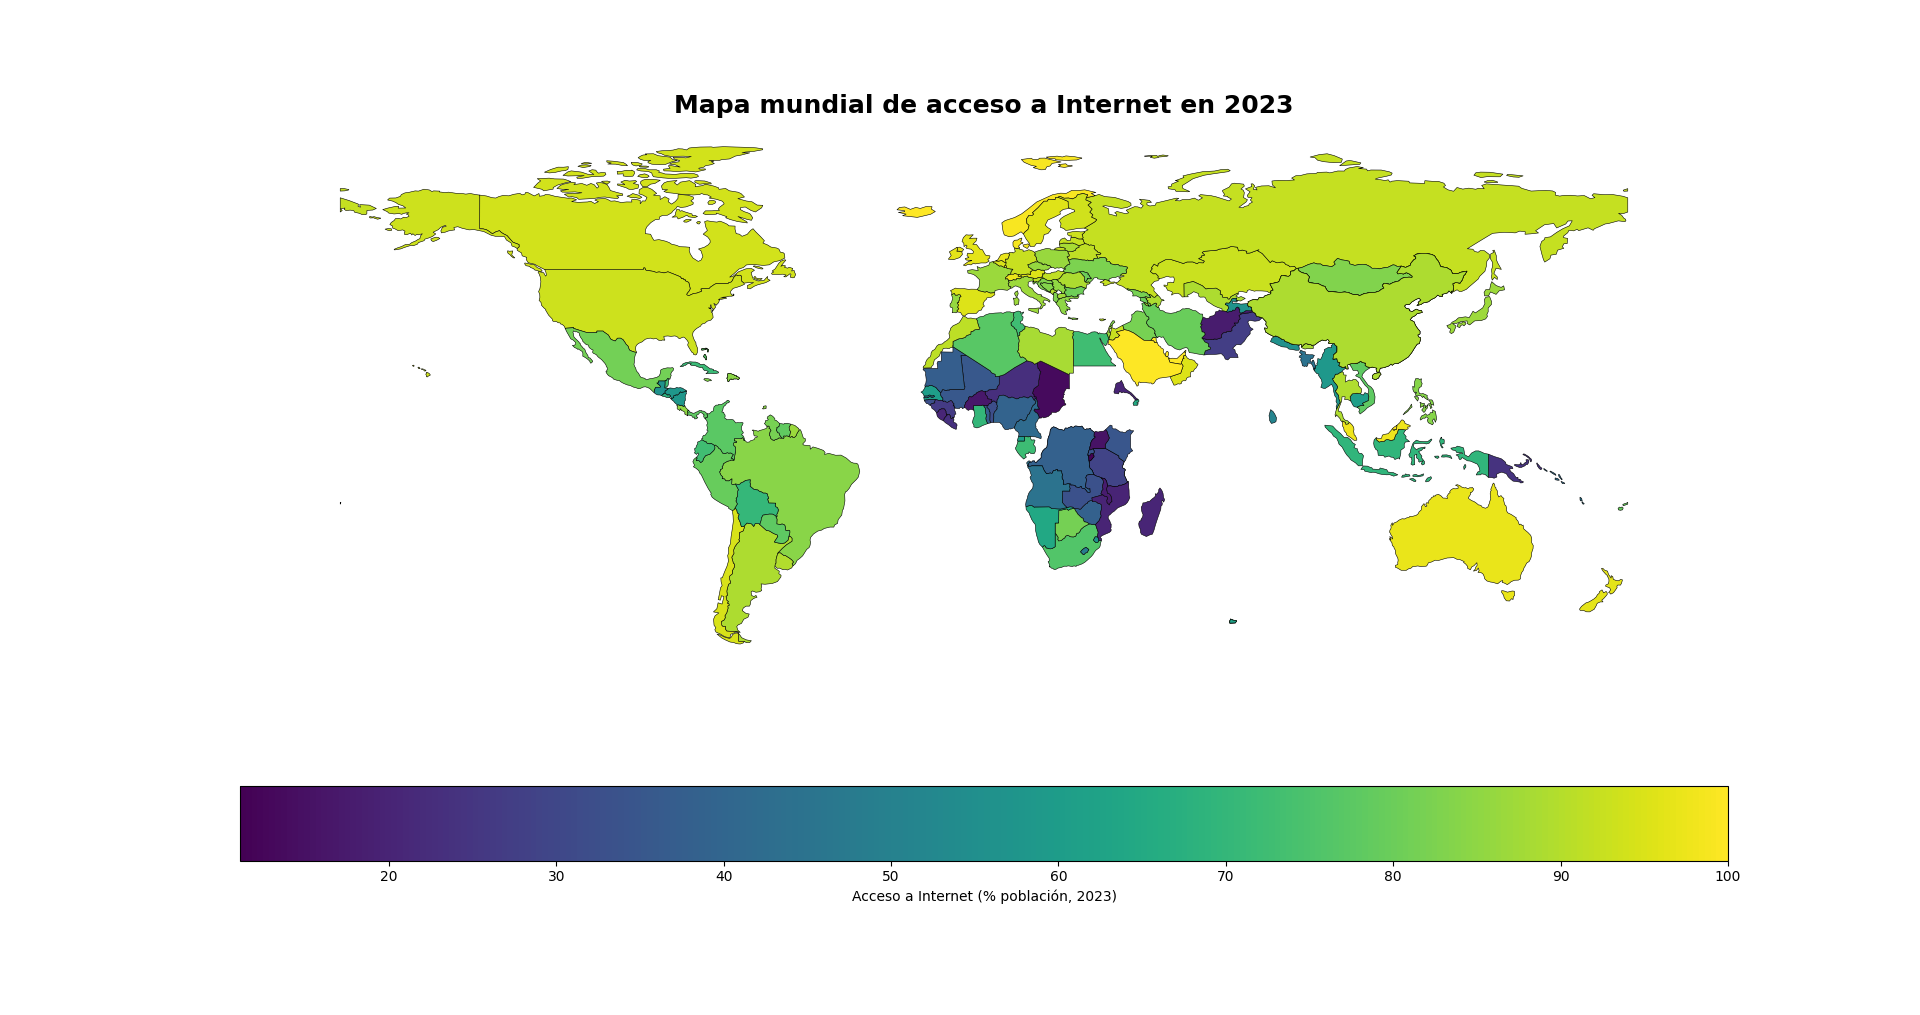
\includegraphics[width=0.85\textwidth]{Graficos/Grafico_uso_de_internet_FC.png}
    \caption[2]{Fuente: Elaboración propia con datos}
\end{figure}

\textbf{Conclusión:}
\begin{itemize}
    \item Se observa que países como Mónaco (56\%), Andorra (52\%) y Liechtenstein (50\%) lideran la contratación de fibra en 2023.
    \item Son en general países pequeños, con economías desarrolladas y buena planificación urbana, lo que facilita la instalación de redes avanzadas.
    \item Países como China, Corea del Sur o Alemania también presentan cifras altas, pero no alcanzan el nivel de penetración de los primeros.
    \item El gráfico también muestra países con niveles más bajos, como Malta y Dinamarca (44\%), lo que sugiere diferencias internas incluso en regiones desarrolladas.
    \item Este tipo de visualización permite un contraste claro de adopción tecnológica y pone en evidencia el avance en infraestructura.
\end{itemize}


% ===================== JAVIER GÓMEZ =====================
\newpage
\subsection*{Integrante 2: Javier Gómez}

\subsubsection*{Criterios Seleccionados}
\begin{itemize}
    \item 
    \item 
\end{itemize}

\subsubsection*{Justificación: }
Permite .

\begin{itemize}
    \item 
    \item 
\end{itemize}

\subsubsection*{Justificación: }
Revela .
\begin{itemize}
    \item 
\end{itemize}

\subsubsection*{Gráfico 3: }
\begin{figure}[H]
    \centering
    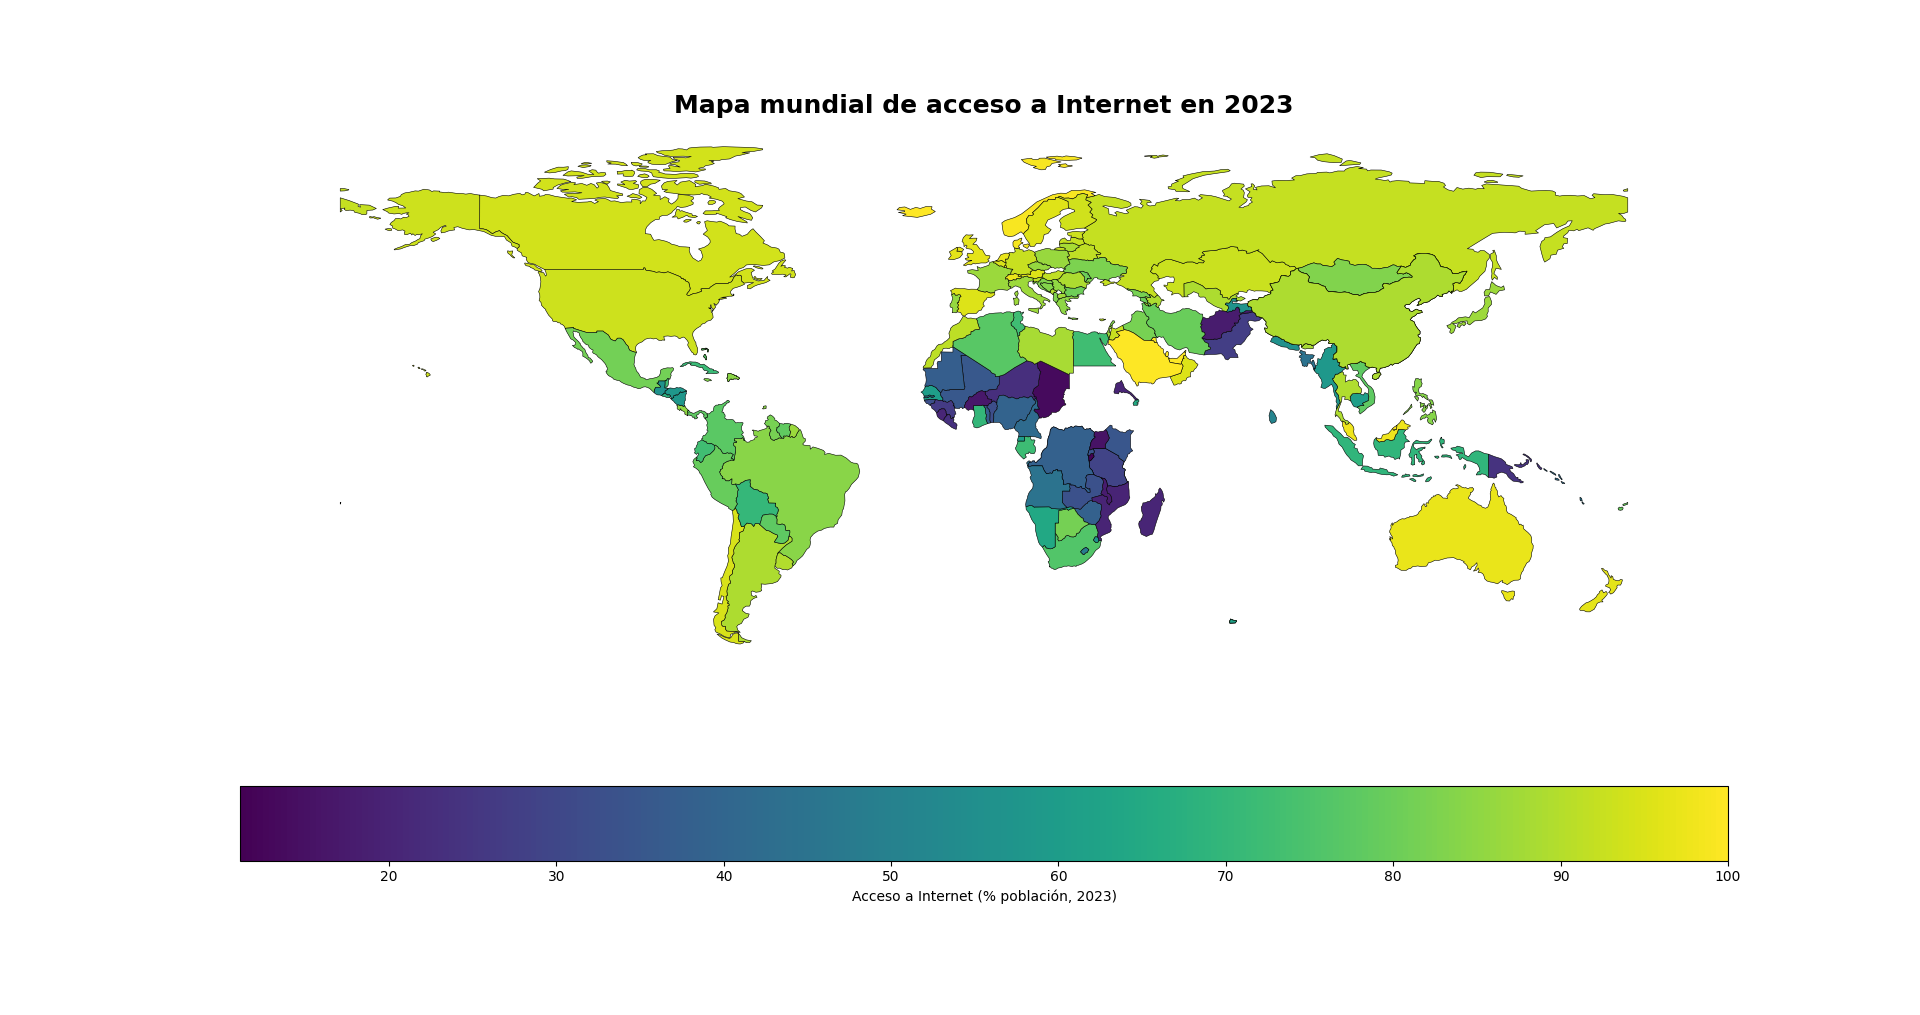
\includegraphics[width=0.85\textwidth]{Graficos/Grafico_uso_de_internet_FC.png}
    \caption[3]{Fuente: Elaboración propia con datos}
\end{figure}

\newpage
\textbf{Conclusión:}  
\begin{itemize}
    \item Como se puede ver en el gráfico, países como Brasil, Nigeria, Filipinas y Chile lideran el ranking en cuanto a uso diario de redes sociales, con promedios superiores a las 3 horas diarias. En general, los países de América Latina y África muestran un uso bastante elevado, lo que refleja lo presentes que están estas plataformas en la vida cotidiana de sus habitantes.
    \item Por otro lado, en países como Japón, Alemania o Bélgica, el tiempo promedio dedicado a redes sociales es mucho menor. Esto puede estar relacionado con diferencias culturales o incluso con estilos de vida donde quizás se priorizan otras formas de comunicación.
    \item El lector podría encontrar interesante realizar un estudio frente a la relación entre cantidad de horas frente a, por ejemplo, rendimiento académico $\bullet{}\bigcirc{}\bullet{}$
\end{itemize}

\subsubsection*{Gráfico 4: }
\begin{figure}[H]
    \centering
    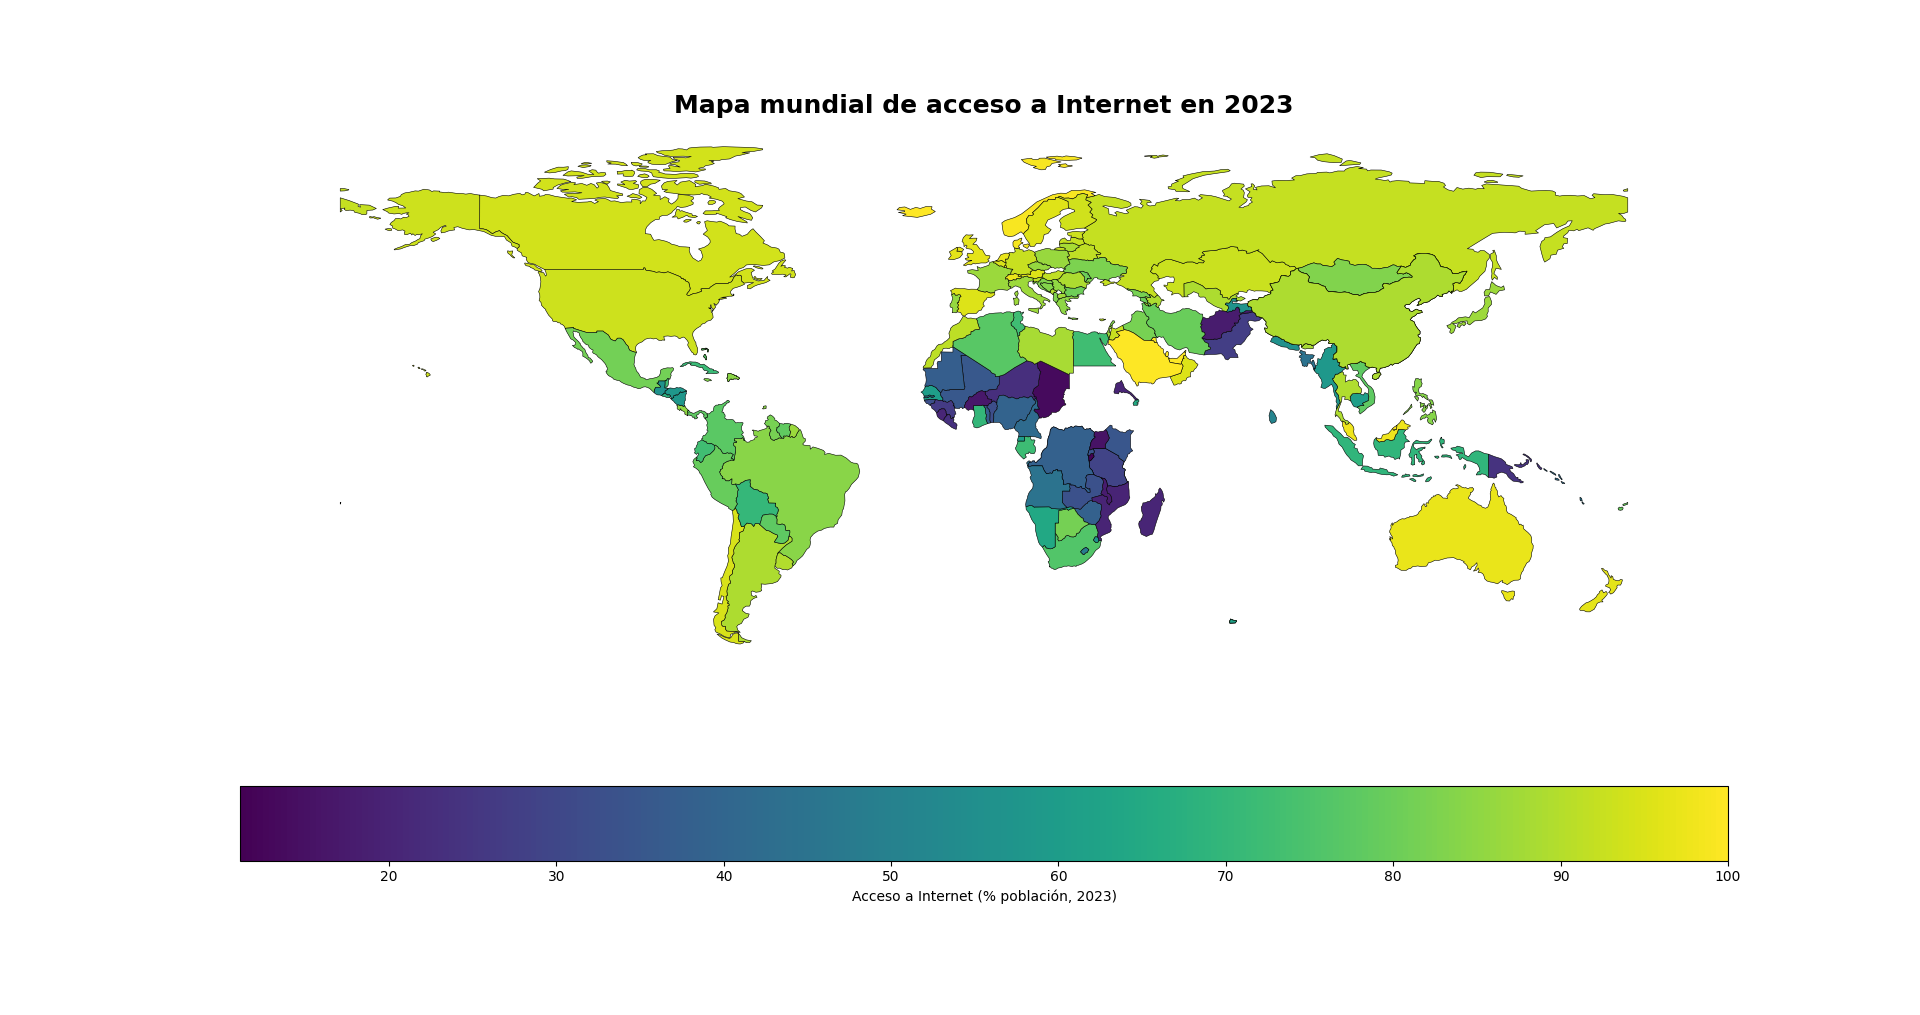
\includegraphics[width=0.85\textwidth]{Graficos/Grafico_uso_de_internet_FC.png}
    \caption[4]{Fuente: Elaboración propia con datos}

\end{figure}


\textbf{Conclusión:}  
\begin{itemize}
    \item Este gráfico muestra la evolución del número de clientes por empresa en los últimos años. Lo más destacable es el aumento significativo de las suscripciones a servicios móviles durante la pandemia \(2020-2021\).
    Durante esos años, varias empresas, como WOM y ENTEL, experimentaron un fuerte crecimiento, probablemente impulsado por la necesidad de mantenerse conectados desde casa, ya sea por trabajo, estudios o simplemente para mantenerse en contacto con los demás.
    \item También es notable cómo algunas empresas han mantenido una base de clientes más estable a lo largo del tiempo, mientras que otras, como VTR Móvil, tienen una participación mucho menor. En 2024, ENTEL se destacó como la empresa con más clientes, superando los 215.000, lo que podría indicar una estrategia comercial sólida o una percepción positiva de su servicio.

\end{itemize}

\begin{figure}[H]
    \centering
    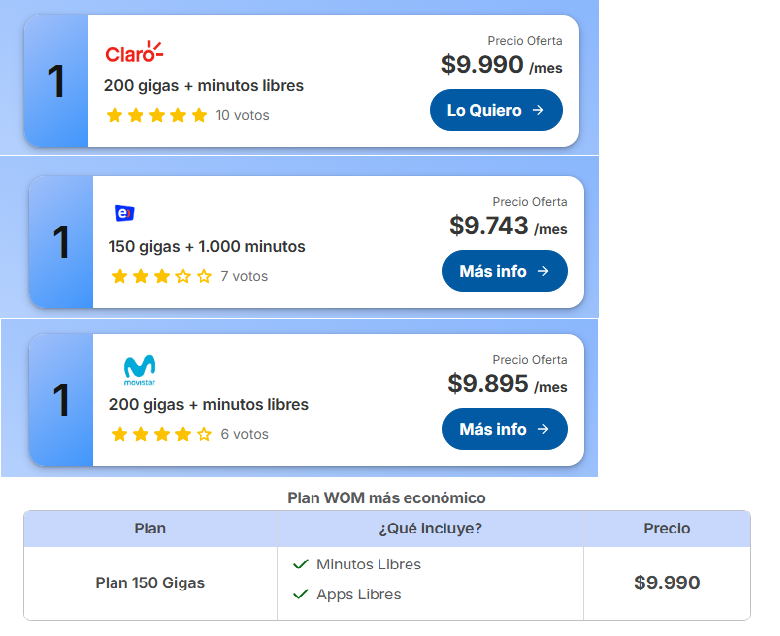
\includegraphics[width=0.85\textwidth]{images/contrastar.png}
    \caption[Relación precio-plan]{
        Comparativa de precios de planes de telefonía móvil entre compañías. \\
        \textbf{Nota:} Es coherente que Entel registre una mayor base de clientes, dado que actualmente ofrece el plan básico más económico del mercado. No obstante, sería interesante contrastar estos datos con los precios de planes de \textit{internet hogar} y \textit{fibra óptica}.%
    }
    \label{fig:precios_telefonia}
    
   
\end{figure}
% ===================== MATÍAS ELGUETA =====================
\subsection*{Integrante 3: Matías Elgueta}

\subsubsection*{Criterios Seleccionados}
\begin{itemize}
    \item Criterio 1: 
    \item Criterio 2: 
\end{itemize}

\subsubsection*{Justificación:}
Nos permite observar cómo es percibida la recolección y utilización de nuestros datos personales por personas de distintas edades, lo que puede ser útil para:

\begin{itemize}
    \item Diseñar campañas de concientización específicas por grupo etario, enfocándose en los públicos que muestran menor preocupación o menor conocimiento sobre el uso de sus datos.
    \item Adaptar políticas de privacidad y términos de uso en plataformas digitales, considerando el nivel de confianza que cada grupo etario tiene respecto al tratamiento de sus datos personales.
\end{itemize}

\subsubsection*{Justificación: Penetracion 5G}
Nos permite visualizar la evolución para la penetración de la red 5G entre 2015 y 2025 en distintos países, lo que facilita la comparación del ritmo de adopción tecnológica a nivel internacional y revela posibles brechas digitales, lo que puede ser útil para:
\begin{itemize}
    \item Tomar decisiones de inversión en infraestructura tecnológica, identificando países con mayor crecimiento 5G, lo cual puede orientar estrategias de empresas del sector de telecomunicaciones.
    \item Diseñar políticas públicas o marcos regulatorios que impulsen una adopción más equitativa de tecnologías avanzadas, especialmente en países con baja penetración, fomentando así la inclusión digital.
\end{itemize}

\subsubsection*{Gráfico 4: Preocupación ante el uso no autorizado de datos personales por rango etario.}
\begin{figure}[H]
    \centering
    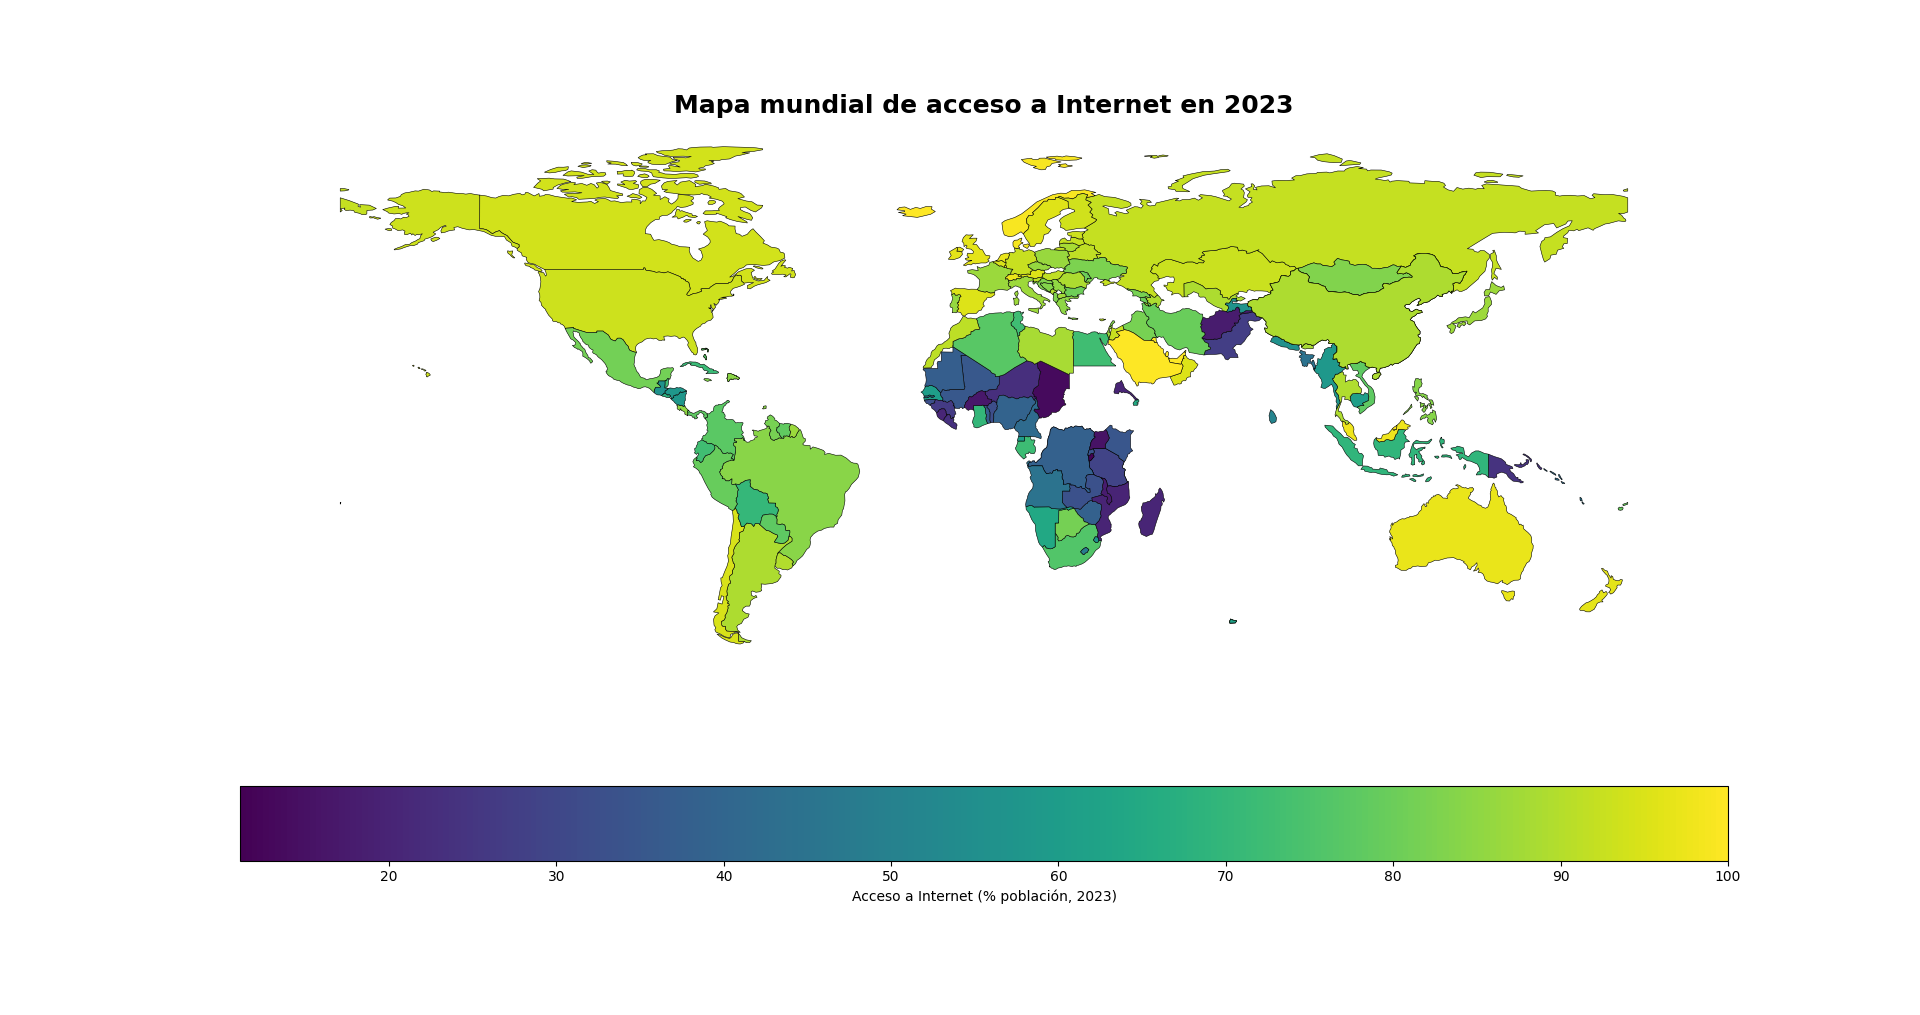
\includegraphics[width=0.85\textwidth]{Graficos/Grafico_uso_de_internet_FC.png}
    \caption[5]{Fuente: Elaboración propia con datos}
\end{figure}

\textbf{Conclusión:}  
\begin{itemize}
    \item Se puede observar una preocupación alta en todos los grupos presentando una mediana cercana a 4 a través de todos los rangos etarios.
    \item Al observar detalladamente cada violín se puede notar que los dos últimos rangos etarios (36-45 y 46+) poseen un valor mínimo de 1, lo que implica que existen encuestados pertenecientes a esos grupos que demuestran la preocupación mínima de 1 respecto al uso de sus datos personales, este no es el caso para los grupos más jóvenes (18-25 y 26-35) donde se observa que incluso los encuestados con menor preocupación poseen por lo menos un nivel ligero de esta.
    \item Junto con esto si nos centramos en los dos últimos grupos etarios, observando cada área, podemos ver que el grupo con edades de 36-45 años son el grupo con la menor preocupación, mostrando también la menor media indicada por la tercera línea horizontal.
\end{itemize}

\subsubsection*{Gráfico 4: Penetracion 5G por país.}
\begin{figure}[H]
    \centering
    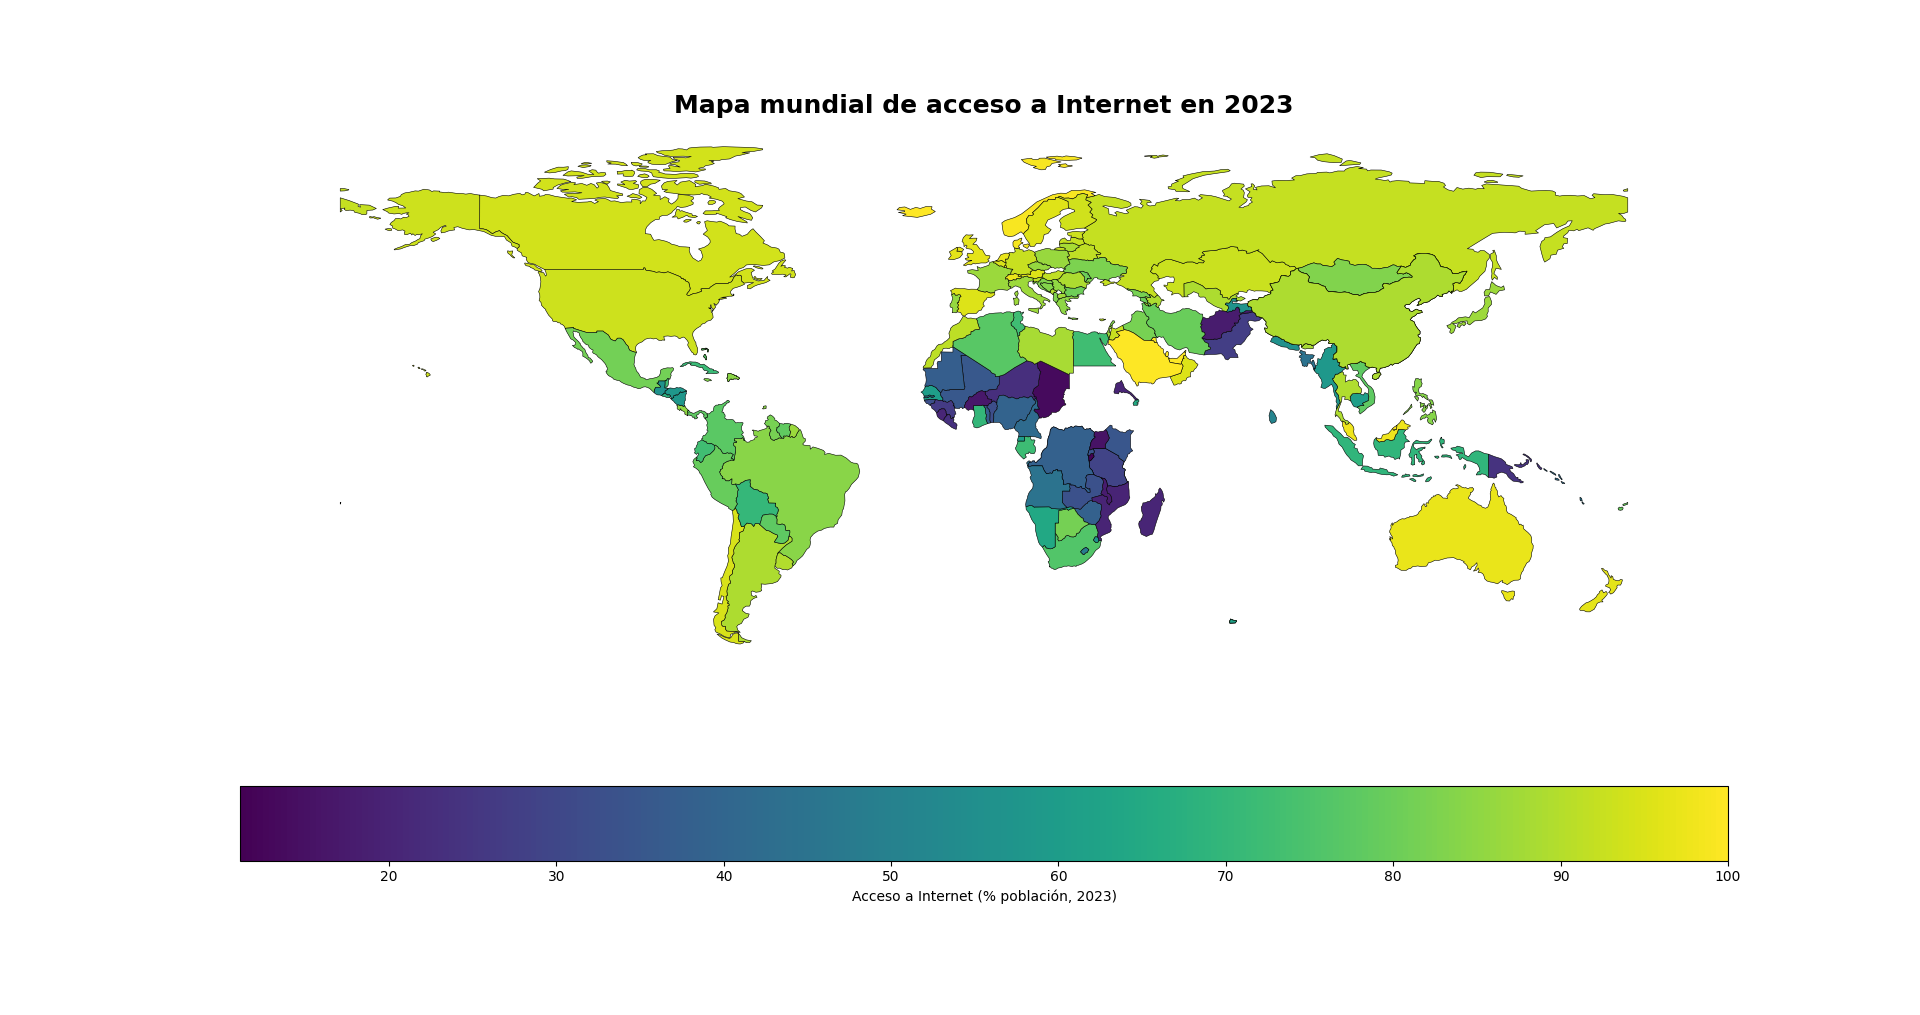
\includegraphics[width=0.85\textwidth]{Graficos/Grafico_uso_de_internet_FC.png}
    \caption[6]{Fuente: Elaboración propia con datos}

\end{figure}


\textbf{Conclusión:}  
\begin{itemize}
    \item Se observa que las curvas suben y bajan visiblemente para casi todos los países, en lugar de crecer de forma sostenida. Esto indica que la penetración 5G ha tenido retrocesos interanuales, lo cual puede deberse a factores técnicos, económicos o políticos que afectan el mantenimiento o la expansión de la red.
    \item Visualmente, países como Francia, Alemania y Japón presentan curvas más suaves y planas, lo cual sugiere un despliegue más progresivo y controlado en comparación con otros países donde hay caídas mas bruscas.

\end{itemize}

% ---------------------------------------------------------------------------------}

\textbf{Repositorio:}  
\label{anexo:repositorio}

Acceso al repositorio en el siguiente link: 
\url{https://github.com/soloimsad/VD.git}

\end{document}
